\section{Proof of Theorem~\ref{thm:gap_B}}

\subsection{Outline}
\label{sec:proof_outline}

We are now prepared to explain the main result.
To study the second largest eigenvalue of the non-backtracking matrix,
we examine the spectral radius of the matrix obtained by subtracting
off the dominant eigenspace.
 We use for this:
\begin{lemma}[\citet*{bordenave2015a}, Lemma 3]
\label{lem:subspace}
Let $T$ and $R$ be matrices such that $\Img(T)\subset \Ker(R)$, 
$\Img(T^*)\subset \Ker(R)$. 
Then all eigenvalues $\lambda$ of $T+R$
that are not eigenvalues of $T$ satisfy:
\[
|\lambda|\leq \max_{x\in \Ker(T)}\frac{\|(T+R)x\|}{\|x\|} .
\]
\end{lemma}
Throughout the text,
$\| \cdot \|$ is the spectral norm for matrices and $\ell^2$-norm for vectors.
Recall that the leading eigenvalues of $B$, in magnitude, are 
$\lambda_1 = \sqrt{(d_1 -1)(d_2-1)}$ and $\lambda_{2|E|} = -\lambda_1$
with corresponding eigenvectors $\1_{\alpha}$ and $\mathbf{1}_{-\alpha}$.
Applying Lemma~\ref{lem:subspace} with 
$T 
= 
\frac{\lambda_1^{\ell}}{\onealpha^* \onealpha}
(\onealpha \onealpha^* +
(-1)^\ell \onemalpha \onemalpha^*)$
and 
$R = B^\ell - T$,
we get that
\begin{align}
\label{eq:upper_bound_lambda2}
\lambda_2(B)
\leq 
\max_{
\footnotesize
\begin{array}{c}
x \in \Ker(T) \\ 
\|x\| = 1 
\end{array}
} 
\left( \| B^{\ell}x \| \right)^{1/\ell}.
\end{align}
It will be important later to have a more precise description of the set $\Ker(T)$. 
It is not hard to check that 
\begin{align*}
\Ker(T) &= \{x:
  ~ \langle x, \onealpha \rangle = \langle x, \onemalpha \rangle=0\} \\
& =\{(v,w)\in \mathbb{R}^{2|E|}: 
  ~ \langle v, \1 \rangle = \langle w, \1 \rangle=0\}.
\end{align*}
In the last line, the vectors $v$, $w$ and $\1$ are $|E|-$dimensional, 
and $\1$ is the vector of all ones.

In order to use Eqn.~\ref{eq:upper_bound_lambda2},
we must bound $\| B^\ell x \|$ for large powers $\ell$
and $x \in \Ker(T)$.
This amounts to counting the contributions of certain non-backtracking walks.
We will use the tangle free property in order to only count
$\ell$-tangle-free walks. 
We break up $B^\ell$ into two parts
in Section~\ref{sec:matrix_decomp}, 
an ``almost'' centered matrix $\bar{B}^\ell$ 
and the remainder $\sum_j R^{\ell,j}$,
and we bound each term independently.

To compute these bounds, 
we need to count the contributions of many different non-backtracking walks.
We will use the trace technique, so only circuits which return to the starting
vertex will contribute. 
In Section~\ref{sec:expectation_bounds},
we compute
the expected contribution of products of $B$ along such circuits, 
employing a result from \cite{bordenave2015}.
% In Section~\ref{sec:expectation_bounds}, 
% we apply a useful result from \citet*{mckay1981a}
% to compute the probability, during the exploration process,
% of revealing a new edge $e$ 
% given that we have already observed a certain subgraph $H$. 
% In particular, we find different probabilities depending on whether $e$
% shares one of more endpoints in $H$.
% We use this to bound the expectation of the of the product of
% entries $\bar{B}_{ef}$ along segments $ef$ of a non-backtracking walk.
% A similar argument appears later, in the proof of Theorem~\ref{spec_R}, 
% for products of $R^{\ell,j}_{ef}$.

Section~\ref{sec:path_counting} covers the combinatorial component of the proof. 
The total contributions $\| B^\ell x \|$ come from many 
non-backtracking circuits of different flavors,
depending on their number of vertices, edges, cycles, etc.
Each circuit is broken up into $2k$ segments of tangle-free
walks of length $\ell$.
We need to compute not only the expectation along the circuit,
but also upper-bound the number of circuits of each flavor.
We introduce an injective
encoding of such circuits that depends on the number of vertices,
length of the circuit, and, crucially, the tree excess of the circuit.
An important part of these calculations is to keep track
of the imbalance between left and right vertices
visited in the circuit, since this controls
the powers of $d_1$ and $d_2$ in the result.

Finally, in Section~\ref{sec:norm_bounds} we put all of these ingredients together
and use Markov's inequality to bound each matrix norm with high probability.
We find that 
$\| \bar{B}^\ell \|$ 
contributes a factor that goes as 
$((d_1 - 1)(d_2 - 1))^{\ell/4}$,
whereas $\| R^{\ell,j} \|$ contributes only a factor of $(d-1)^\ell/n$,
up to polylogarithmic factors in $n$.
Thus, the main contribution to the circuit counts comes from the mean
and, in fact, comes from circuits which are exactly trees traversed 
forwards and backwards.
Interestingly, this
is analogous to what happens when using the trace method
on random matrices of independent entries. 

In the proof, we are forced to consider tangled paths
but which are built up of tangle-free components.
This delicate issue was first made clear by \citet*{friedman2004}
who introduced the idea of tangles and a ``selective trace.''
\citet*{bordenave2015a}, who we follow closely in this part of our analysis,
also has a good discussion of these issues and their history.
We use the fact that
\begin{equation}
\label{eq:trace_bound}
\E\left(\|\bar{B}^{\ell}\|^{2k}\right)
\leq 
\E\left( 
\mathrm{Tr} 
\left[
\left( (\bar{B}^{\ell}) (\bar{B}^{\ell})^* \right)^{k} 
\right]
\right),
\end{equation}
and so deal with circuits built up of $2k$ segments which are $\ell$-tangle-free.
Notice that the first segment comes from $\bar{B}^\ell$, the second
from $(\bar{B}^{\ell})^*$, etc.
Because of this, the directionality of the edges along each segment alternates.
See Figure~\ref{fig:circuit} for an illustration of a path
which contributes for $k=2$ and $\ell=2$.
Also, while each segment is $\ell$-tangle-free,
the overall circuit may be tangled.

\begin{figure}[t!]
\centering
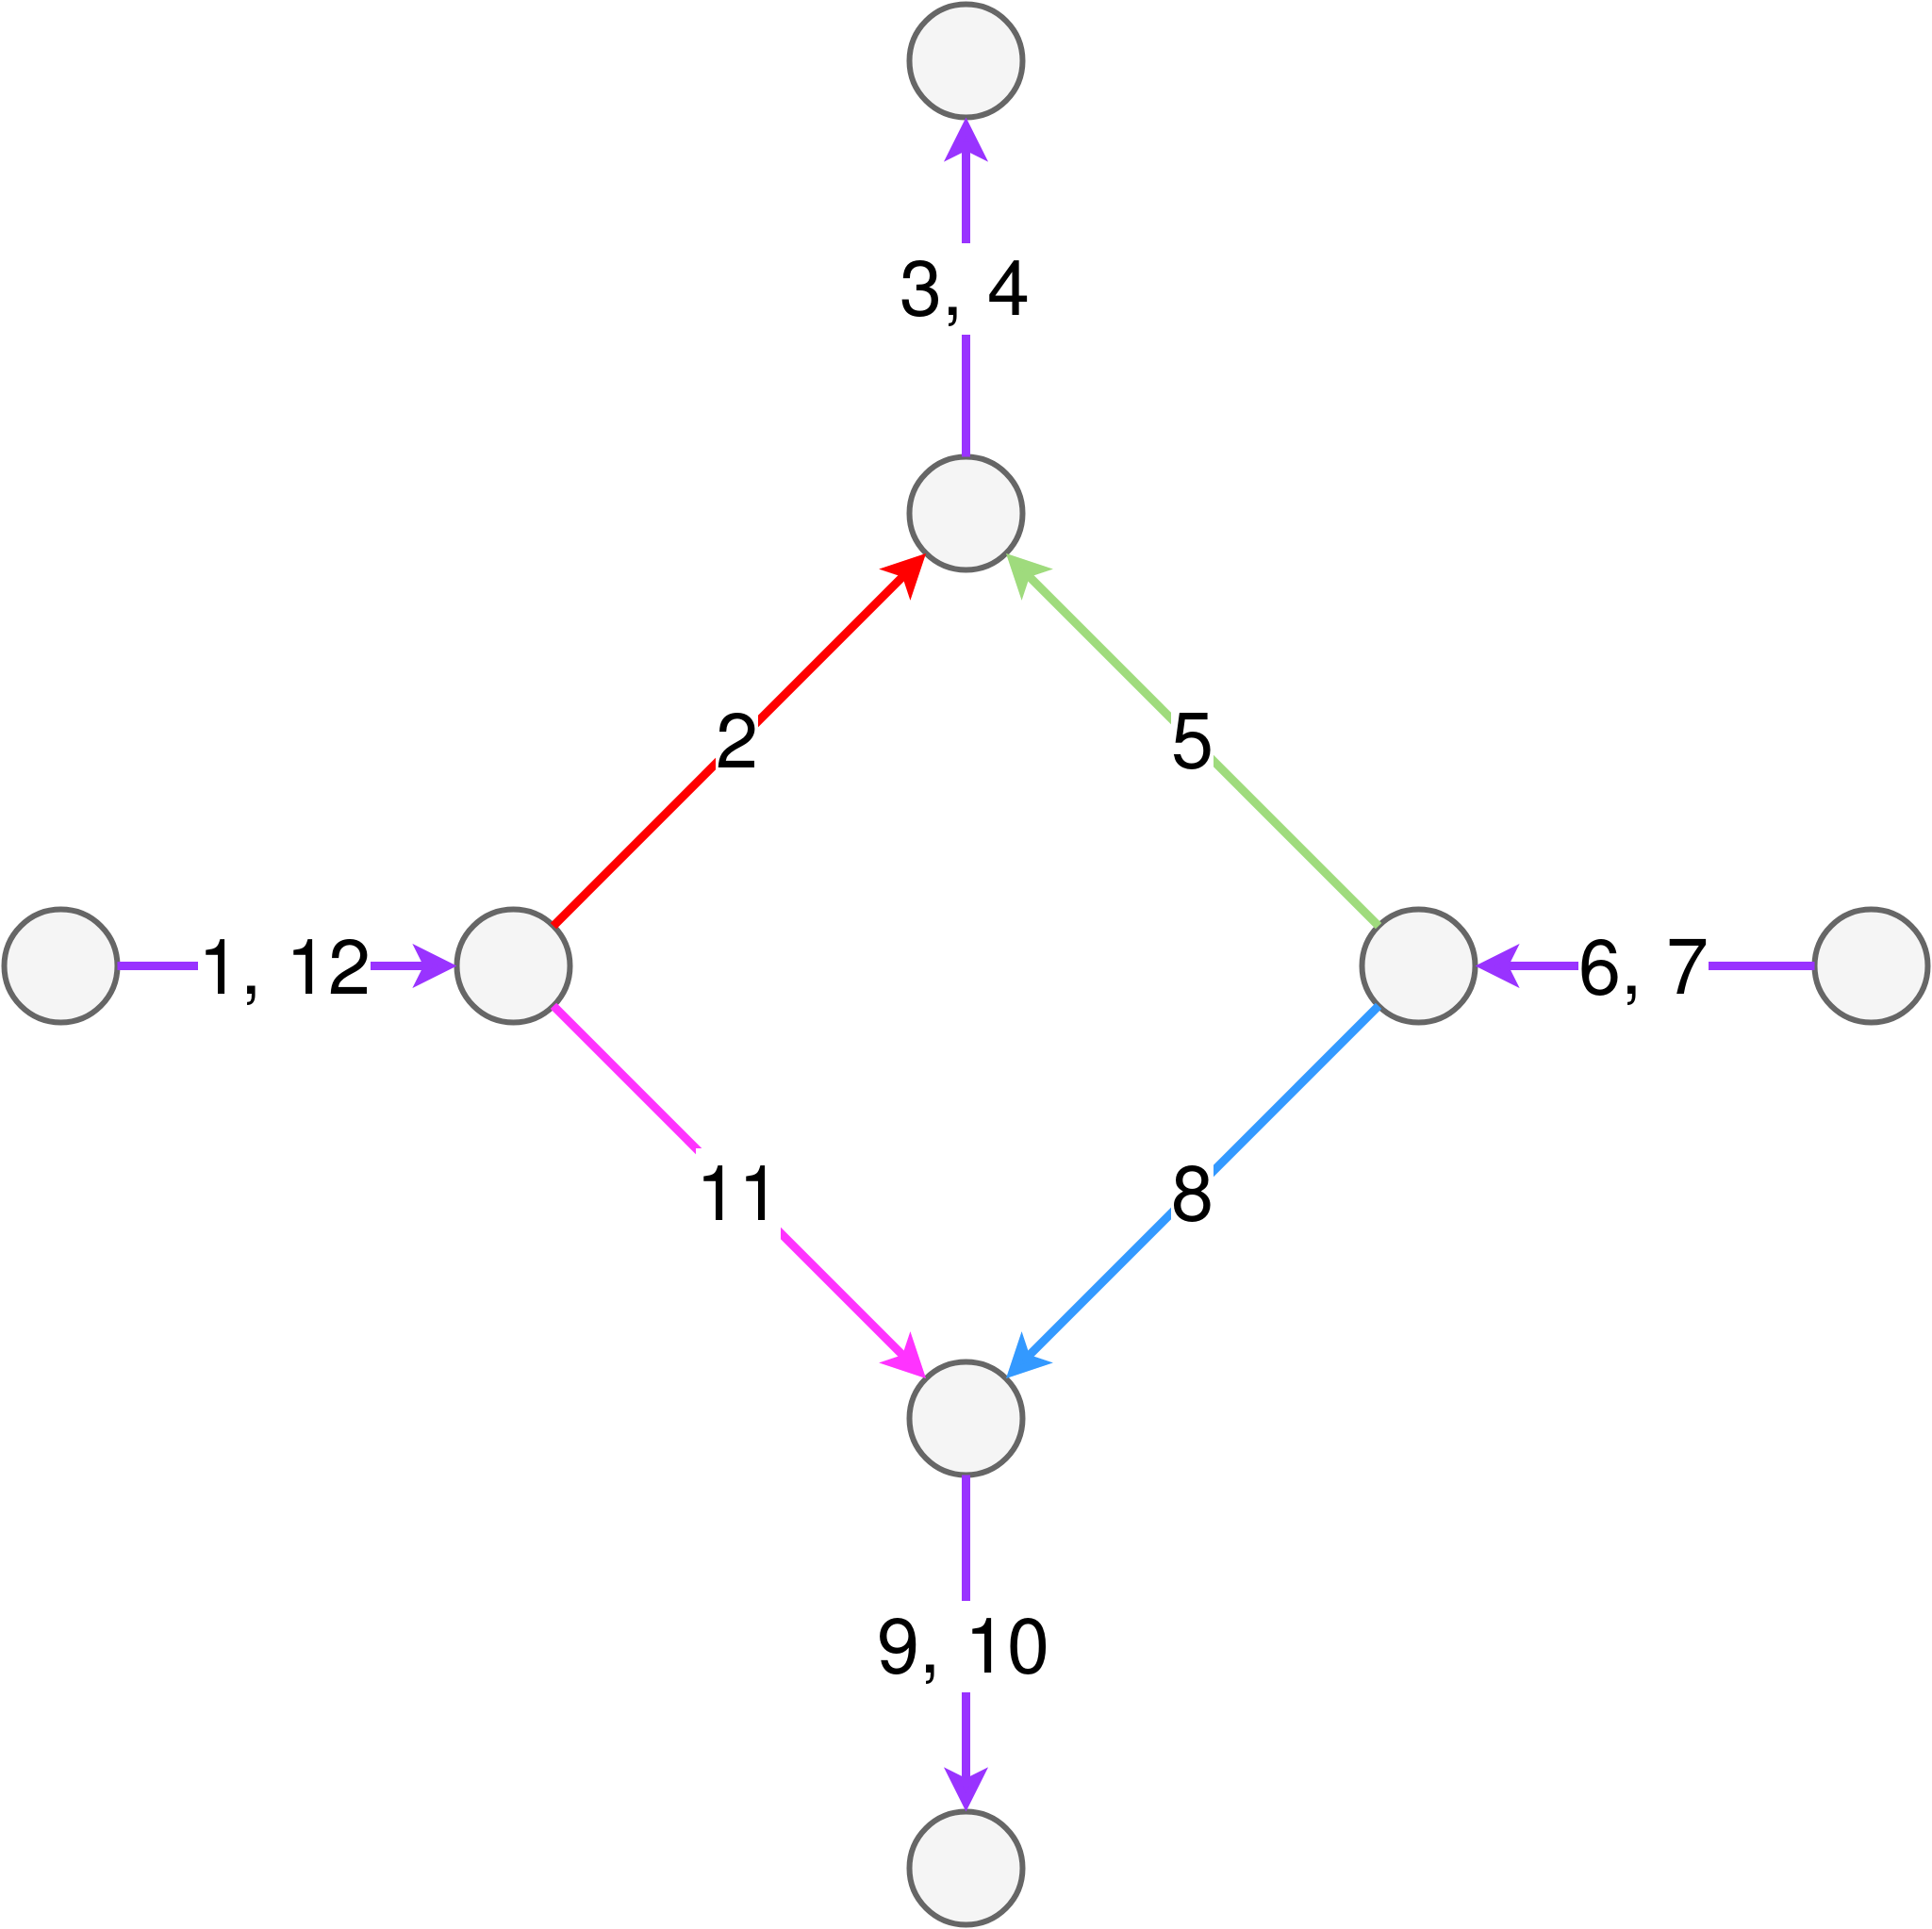
\includegraphics[width=0.4\linewidth]{circuit_k_2_l_2.png}

\caption{An example circuit that contributes to the trace in 
	Eqn.~\eqref{eq:trace_bound},
 for $k = 2$ and $\ell = 2$.
 Edges are numbered as they occur in the circuit.
 Each segment $\{ \gamma_i \}_{i=1}^4$ 
 is of length $\ell + 1 = 3$ and made up of edges $3(i-1)+1$ through $3i$.
 The last edge of each $\gamma_i$ is the first edge of $\gamma_{i+1}$, 
 and these are shown in purple.
 Every path $\gamma_{i}$ with $i$ even
 follows the edges backwards due to the matrix transpose.
 However, this detail turns out not to make any difference since the underlying
 graph is undirected.
 Our example has no cycles in each segment for clarity,
 but, in general, each segment can have up to one cycle, 
 and the overall circuit may be tangled.
}
\label{fig:circuit}
\end{figure}









